\subsection{Aufnahme der Hysterese}
Die gemessenen magnetischen Flussdichten $B$ in Abhängigkeit der angelegten Stromstärke $I$
sind in Tabelle \ref{tab: hysterese} aufgetragen. Eine graphische Darstellung befindet sich in Abbildung
\ref{fig: hysterese_gesamt}. Mittels der Messwerte wird eine Regression nach dem Prinzip der kleinsten Quadrate
an eine Funktion der Form
\begin{equation}
  B(I) = a_1 I^3 + a_2 I^2 + a_3 I ^2 + a_4
  \label{eq: fitfuntion_hysterese}
\end{equation}
bestimmt. Für den austeigenden Ast der Hysterese ergeben sich folgende Parameter
\begin{align}
  \begin{aligned}
    a_1 &= \SI{-0.7(1)e-1}{\milli\tesla \per \ampere ^3} & a_2 &= \SI{1.5(3)}{\milli\tesla \per \ampere ^2} \\
    a_3 &= \SI{5.1(3)e1}{\milli\tesla \per \ampere } & a_4 &= \SI{3(6)}{\milli\tesla }.
    \label{eq: params_up}
  \end{aligned}
\end{align}
Analog werden folgende Werte für den absteigenden Ast gefunden
\begin{align}
  \begin{aligned}
    b_1 &= \SI{-8.6(8)e-2}{\milli\tesla \per \ampere ^3} & b_2 &= \SI{1.9(3)}{\milli\tesla \per \ampere ^2} \\
    b_3 &= \SI{4.7(2)e1}{\milli\tesla \per \ampere } & b_4 &= \SI{11(4)}{\milli\tesla }.
  \end{aligned}
\end{align}
Eine graphische Darstellung der Fitfunktionen befindet sich in Abbildung \ref{fig: hysterese_fit}.
\subsection{Aufnahme der Hysterese}
Die gemessenen magnetischen Flussdichten $B$ in Abhängigkeit der angelegten Stromstärke $I$
sind in Tabelle \ref{tab: hysterese} aufgetragen. Eine graphische Darstellung befindet sich in Abbildung
\ref{fig: hysterese_gesamt}. Mittels der Messwerte wird eine Regression nach dem Prinzip der kleinsten Quadrate
an eine Funktion der Form
\begin{equation}
  B(I) = a_1 I^3 + a_2 I^2 + a_3 I ^2 + a_4
  \label{eq: fitfuntion_hysterese}
\end{equation}
bestimmt. Für den austeigenden Ast der Hysterese ergeben sich folgende Parameter
\begin{align}
  \begin{aligned}
    a_1 &= \SI{-0.7(1)e-1}{\milli\tesla \per \ampere ^3} & a_2 &= \SI{1.5(3)}{\milli\tesla \per \ampere ^2} \\
    a_3 &= \SI{5.1(3)e1}{\milli\tesla \per \ampere } & a_4 &= \SI{3(6)}{\milli\tesla }.
    \label{eq: params_up}
  \end{aligned}
\end{align}
Analog werden folgende Werte für den absteigenden Ast gefunden
\begin{align}
  \begin{aligned}
    b_1 &= \SI{-8.6(8)e-2}{\milli\tesla \per \ampere ^3} & b_2 &= \SI{1.9(3)}{\milli\tesla \per \ampere ^2} \\
    b_3 &= \SI{4.7(2)e1}{\milli\tesla \per \ampere } & b_4 &= \SI{11(4)}{\milli\tesla }.
  \end{aligned}
\end{align}
Eine graphische Darstellung der Fitfunktionen befindet sich in Abbildung \ref{fig: hysterese_fit}.
\subsection{Aufnahme der Hysterese}
Die gemessenen magnetischen Flussdichten $B$ in Abhängigkeit der angelegten Stromstärke $I$
sind in Tabelle \ref{tab: hysterese} aufgetragen. Eine graphische Darstellung befindet sich in Abbildung
\ref{fig: hysterese_gesamt}. Mittels der Messwerte wird eine Regression nach dem Prinzip der kleinsten Quadrate
an eine Funktion der Form
\begin{equation}
  B(I) = a_1 I^3 + a_2 I^2 + a_3 I ^2 + a_4
  \label{eq: fitfuntion_hysterese}
\end{equation}
bestimmt. Für den austeigenden Ast der Hysterese ergeben sich folgende Parameter
\begin{align}
  \begin{aligned}
    a_1 &= \SI{-0.7(1)e-1}{\milli\tesla \per \ampere ^3} & a_2 &= \SI{1.5(3)}{\milli\tesla \per \ampere ^2} \\
    a_3 &= \SI{5.1(3)e1}{\milli\tesla \per \ampere } & a_4 &= \SI{3(6)}{\milli\tesla }.
    \label{eq: params_up}
  \end{aligned}
\end{align}
Analog werden folgende Werte für den absteigenden Ast gefunden
\begin{align}
  \begin{aligned}
    b_1 &= \SI{-8.6(8)e-2}{\milli\tesla \per \ampere ^3} & b_2 &= \SI{1.9(3)}{\milli\tesla \per \ampere ^2} \\
    b_3 &= \SI{4.7(2)e1}{\milli\tesla \per \ampere } & b_4 &= \SI{11(4)}{\milli\tesla }.
  \end{aligned}
\end{align}
Eine graphische Darstellung der Fitfunktionen befindet sich in Abbildung \ref{fig: hysterese_fit}.
\subsection{Aufnahme der Hysterese}
Die gemessenen magnetischen Flussdichten $B$ in Abhängigkeit der angelegten Stromstärke $I$
sind in Tabelle \ref{tab: hysterese} aufgetragen. Eine graphische Darstellung befindet sich in Abbildung
\ref{fig: hysterese_gesamt}. Mittels der Messwerte wird eine Regression nach dem Prinzip der kleinsten Quadrate
an eine Funktion der Form
\begin{equation}
  B(I) = a_1 I^3 + a_2 I^2 + a_3 I ^2 + a_4
  \label{eq: fitfuntion_hysterese}
\end{equation}
bestimmt. Für den austeigenden Ast der Hysterese ergeben sich folgende Parameter
\begin{align}
  \begin{aligned}
    a_1 &= \SI{-0.7(1)e-1}{\milli\tesla \per \ampere ^3} & a_2 &= \SI{1.5(3)}{\milli\tesla \per \ampere ^2} \\
    a_3 &= \SI{5.1(3)e1}{\milli\tesla \per \ampere } & a_4 &= \SI{3(6)}{\milli\tesla }.
    \label{eq: params_up}
  \end{aligned}
\end{align}
Analog werden folgende Werte für den absteigenden Ast gefunden
\begin{align}
  \begin{aligned}
    b_1 &= \SI{-8.6(8)e-2}{\milli\tesla \per \ampere ^3} & b_2 &= \SI{1.9(3)}{\milli\tesla \per \ampere ^2} \\
    b_3 &= \SI{4.7(2)e1}{\milli\tesla \per \ampere } & b_4 &= \SI{11(4)}{\milli\tesla }.
  \end{aligned}
\end{align}
Eine graphische Darstellung der Fitfunktionen befindet sich in Abbildung \ref{fig: hysterese_fit}.
\input{../Messdaten/tabs/hysterese.tex}
\begin{figure}
  \centering
  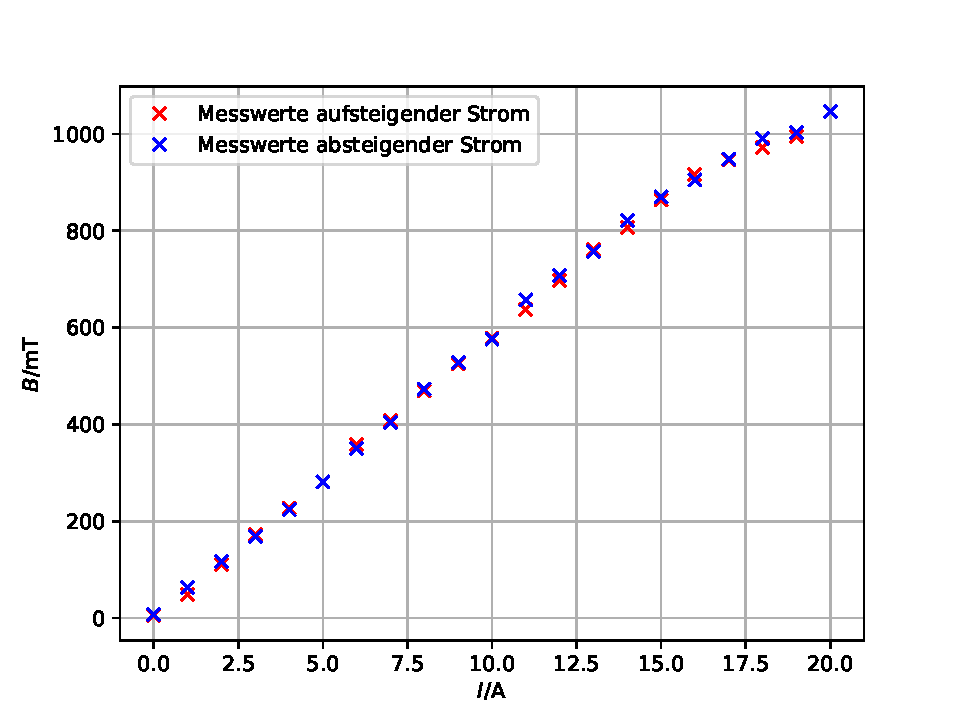
\includegraphics[width = \textwidth]{../Messdaten/plots/hysterese_data.pdf}
  \caption{Graphische Darstellung der Messwerte zur Bestimmung des Zusammenhangs $B(I)$ zwischen angelegtem Strom $I$ und
  magnetischer Flussdichte $B$ des Elektromagneten.}
  \label{fig: hysterese_gesamt}
\end{figure}
\begin{figure}
  \centering
  \begin{subfigure}{0.48\textwidth}
    \centering
  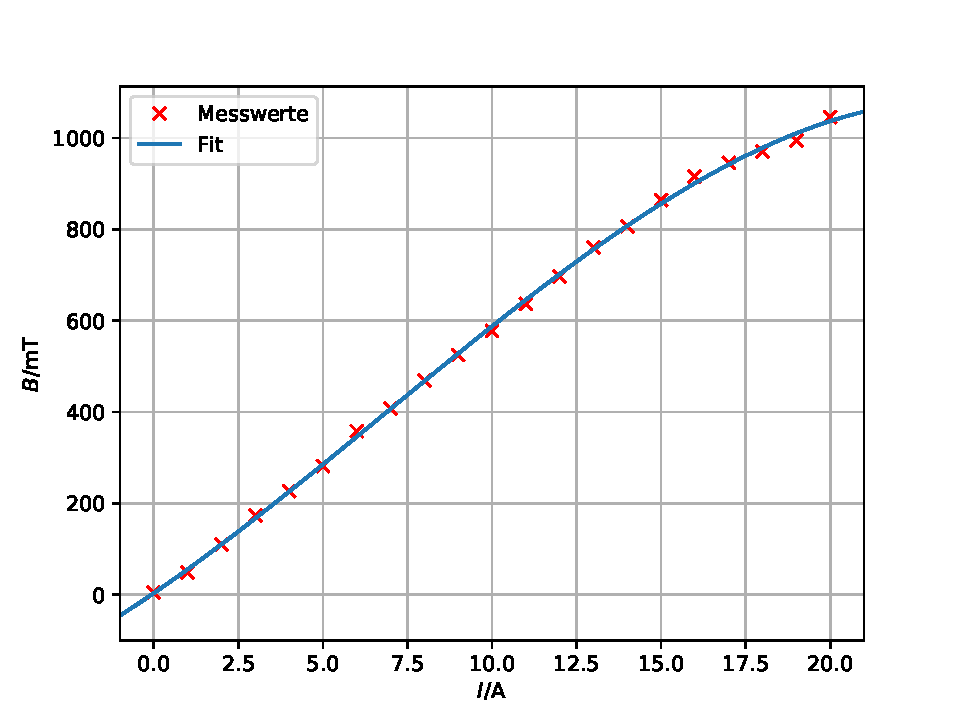
\includegraphics[width = \textwidth]{../Messdaten/plots/hysterese_aufsteigend.pdf}
  \caption{Aufsteigender Strom $I$.}
  \label{fig: hysterese_aufsteigend}
\end{subfigure}
\hfill
  \begin{subfigure}{0.48\textwidth}
  \centering
  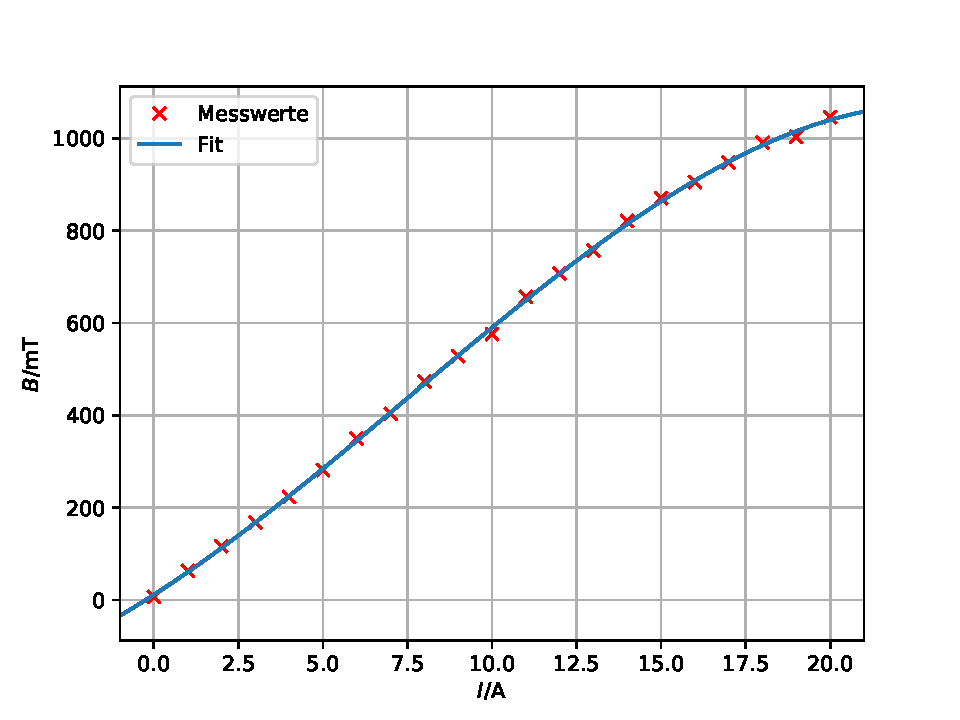
\includegraphics[width = \textwidth]{../Messdaten/plots/hysterese_absteigend.pdf}
  \caption{Absteigender Strom $I$.}
  \label{fig: hysterese_absteigend}
\end{subfigure}
\caption{Graphische Darstellung der Abhängigkeit $B(I)$ unter ab-/aufsteigendem Strom $I$ mit jeweiliger Regressionskurve.}
\label{fig: hysterese_fit}
\end{figure}
Im Folgenden wird Gleichung \eqref{eq: fitfuntion_hysterese} mit den Parametern \eqref{eq: params_up}
verwendet um den notwendigen Zusammenhang zwischen angelegtem Strom $I$ und magnetischer Flussdichte $B$ herzustellen.

\begin{figure}
  \centering
  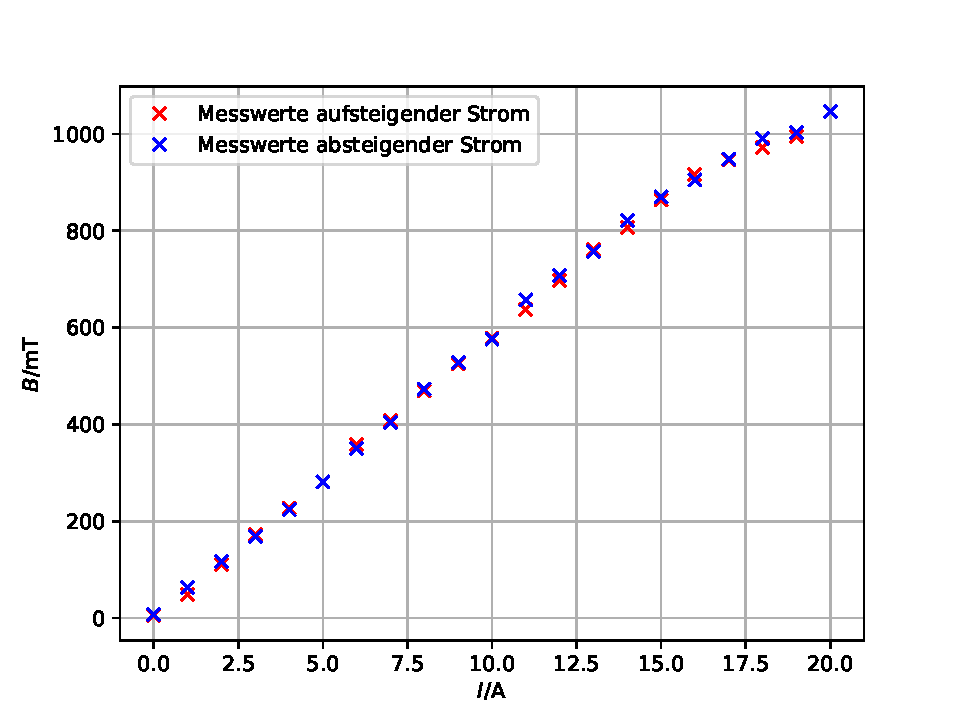
\includegraphics[width = \textwidth]{../Messdaten/plots/hysterese_data.pdf}
  \caption{Graphische Darstellung der Messwerte zur Bestimmung des Zusammenhangs $B(I)$ zwischen angelegtem Strom $I$ und
  magnetischer Flussdichte $B$ des Elektromagneten.}
  \label{fig: hysterese_gesamt}
\end{figure}
\begin{figure}
  \centering
  \begin{subfigure}{0.48\textwidth}
    \centering
  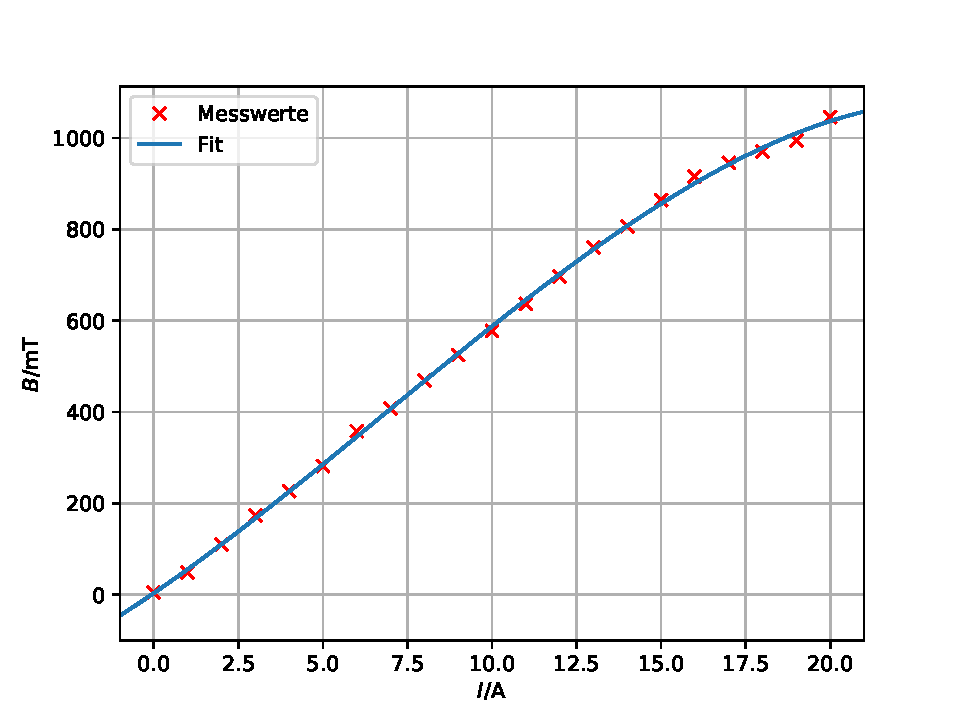
\includegraphics[width = \textwidth]{../Messdaten/plots/hysterese_aufsteigend.pdf}
  \caption{Aufsteigender Strom $I$.}
  \label{fig: hysterese_aufsteigend}
\end{subfigure}
\hfill
  \begin{subfigure}{0.48\textwidth}
  \centering
  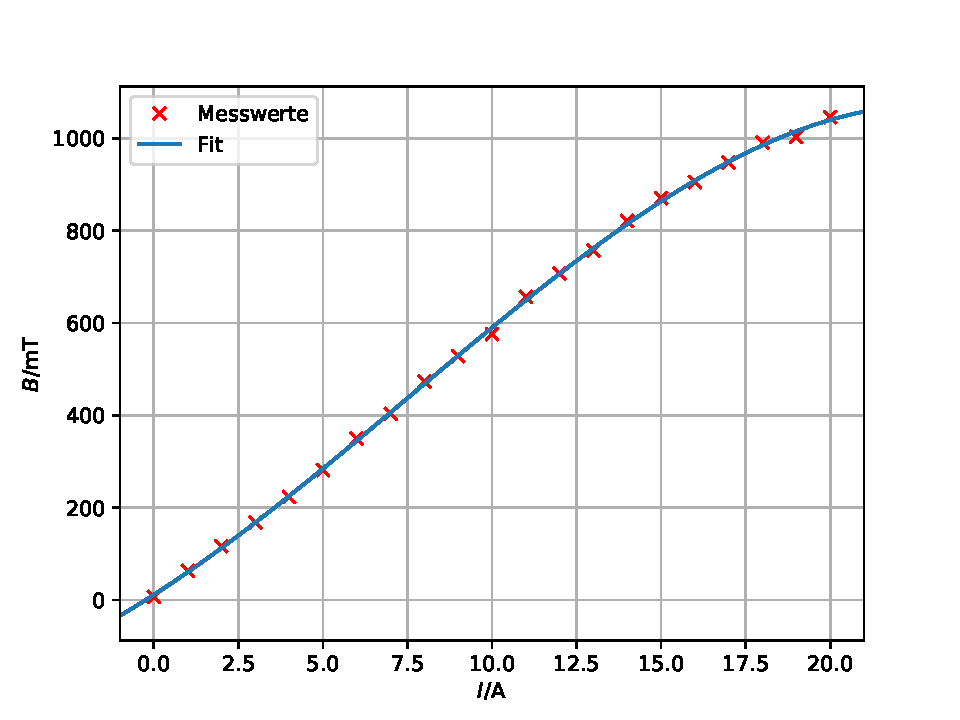
\includegraphics[width = \textwidth]{../Messdaten/plots/hysterese_absteigend.pdf}
  \caption{Absteigender Strom $I$.}
  \label{fig: hysterese_absteigend}
\end{subfigure}
\caption{Graphische Darstellung der Abhängigkeit $B(I)$ unter ab-/aufsteigendem Strom $I$ mit jeweiliger Regressionskurve.}
\label{fig: hysterese_fit}
\end{figure}
Im Folgenden wird Gleichung \eqref{eq: fitfuntion_hysterese} mit den Parametern \eqref{eq: params_up}
verwendet um den notwendigen Zusammenhang zwischen angelegtem Strom $I$ und magnetischer Flussdichte $B$ herzustellen.

\begin{figure}
  \centering
  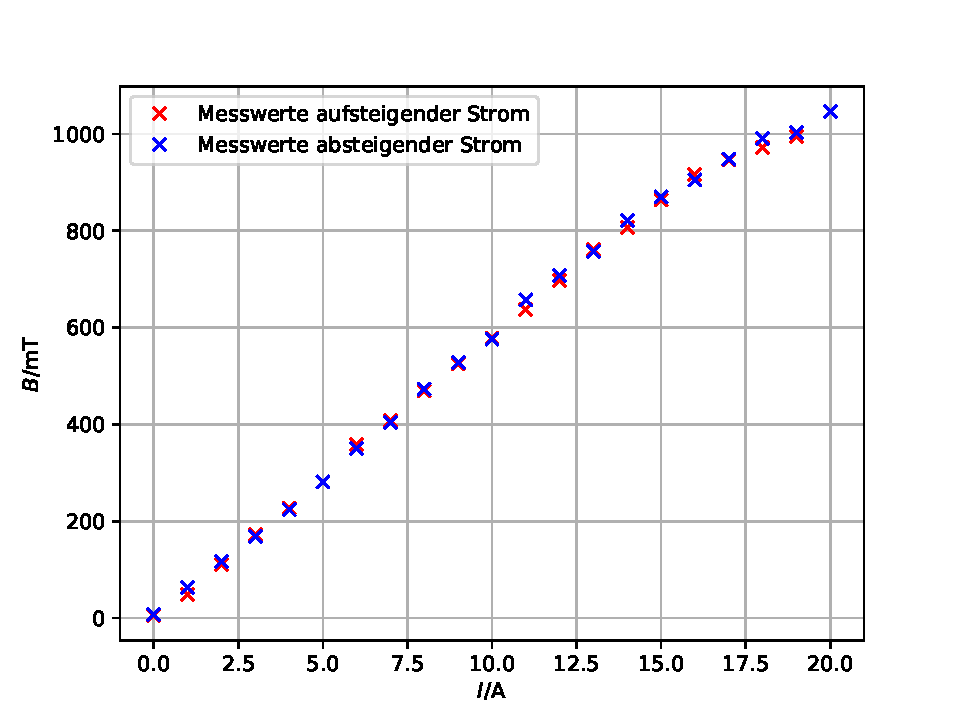
\includegraphics[width = \textwidth]{../Messdaten/plots/hysterese_data.pdf}
  \caption{Graphische Darstellung der Messwerte zur Bestimmung des Zusammenhangs $B(I)$ zwischen angelegtem Strom $I$ und
  magnetischer Flussdichte $B$ des Elektromagneten.}
  \label{fig: hysterese_gesamt}
\end{figure}
\begin{figure}
  \centering
  \begin{subfigure}{0.48\textwidth}
    \centering
  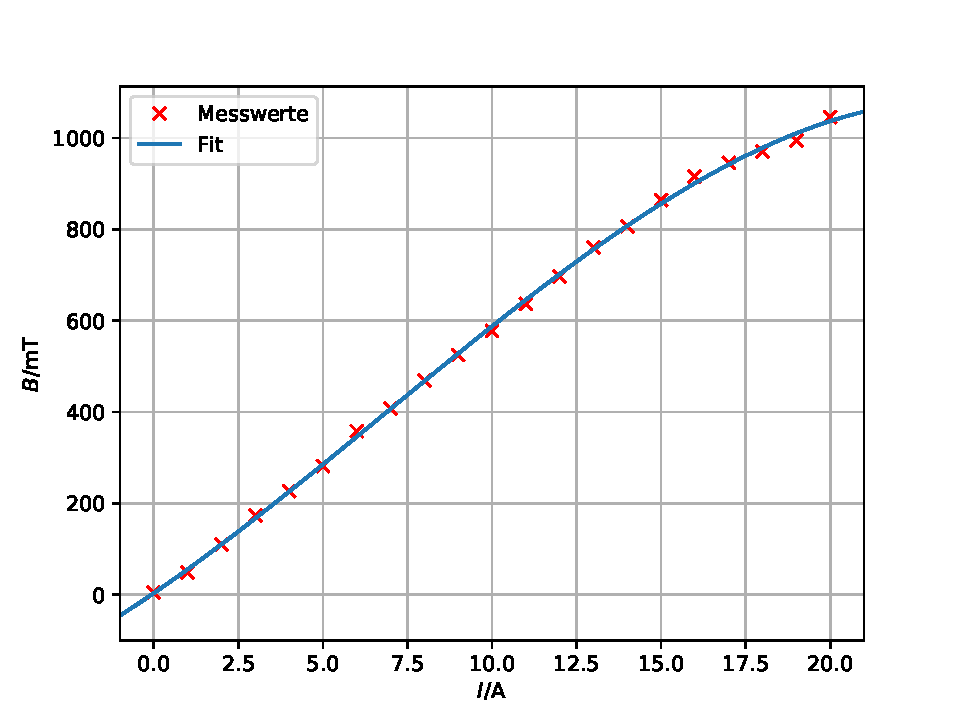
\includegraphics[width = \textwidth]{../Messdaten/plots/hysterese_aufsteigend.pdf}
  \caption{Aufsteigender Strom $I$.}
  \label{fig: hysterese_aufsteigend}
\end{subfigure}
\hfill
  \begin{subfigure}{0.48\textwidth}
  \centering
  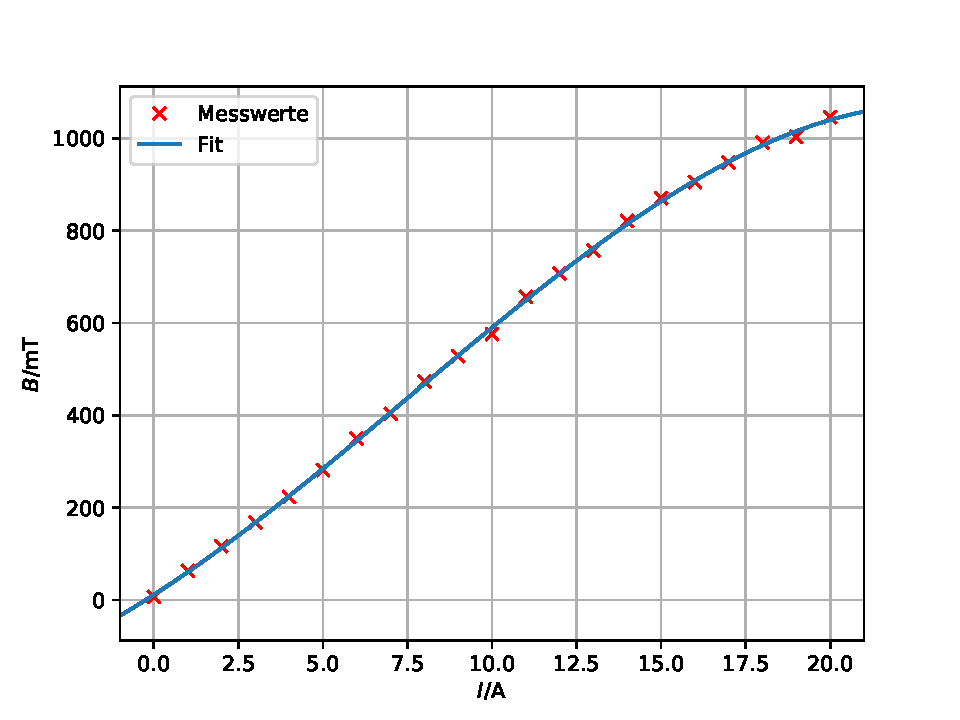
\includegraphics[width = \textwidth]{../Messdaten/plots/hysterese_absteigend.pdf}
  \caption{Absteigender Strom $I$.}
  \label{fig: hysterese_absteigend}
\end{subfigure}
\caption{Graphische Darstellung der Abhängigkeit $B(I)$ unter ab-/aufsteigendem Strom $I$ mit jeweiliger Regressionskurve.}
\label{fig: hysterese_fit}
\end{figure}
Im Folgenden wird Gleichung \eqref{eq: fitfuntion_hysterese} mit den Parametern \eqref{eq: params_up}
verwendet um den notwendigen Zusammenhang zwischen angelegtem Strom $I$ und magnetischer Flussdichte $B$ herzustellen.

\begin{figure}
  \centering
  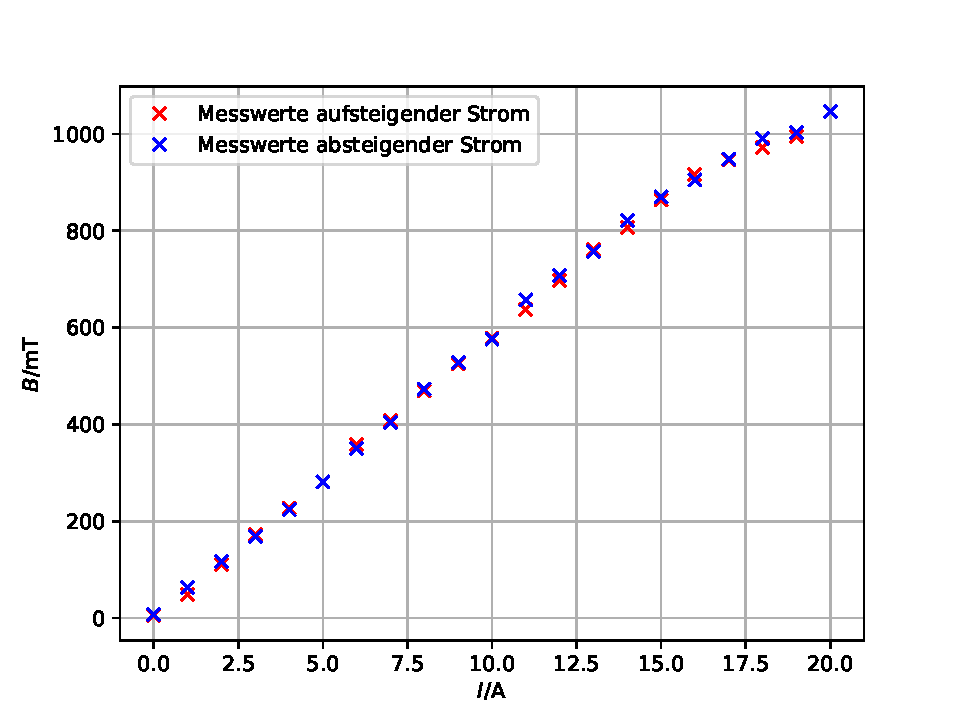
\includegraphics[width = \textwidth]{../Messdaten/plots/hysterese_data.pdf}
  \caption{Graphische Darstellung der Messwerte zur Bestimmung des Zusammenhangs $B(I)$ zwischen angelegtem Strom $I$ und
  magnetischer Flussdichte $B$ des Elektromagneten.}
  \label{fig: hysterese_gesamt}
\end{figure}
\begin{figure}
  \centering
  \begin{subfigure}{0.48\textwidth}
    \centering
  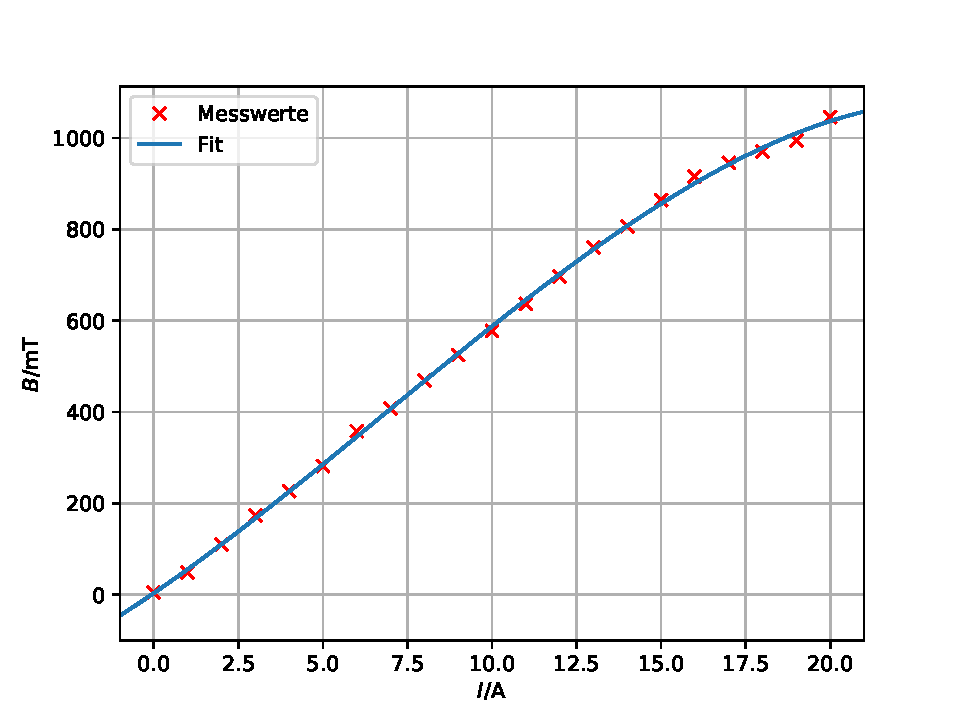
\includegraphics[width = \textwidth]{../Messdaten/plots/hysterese_aufsteigend.pdf}
  \caption{Aufsteigender Strom $I$.}
  \label{fig: hysterese_aufsteigend}
\end{subfigure}
\hfill
  \begin{subfigure}{0.48\textwidth}
  \centering
  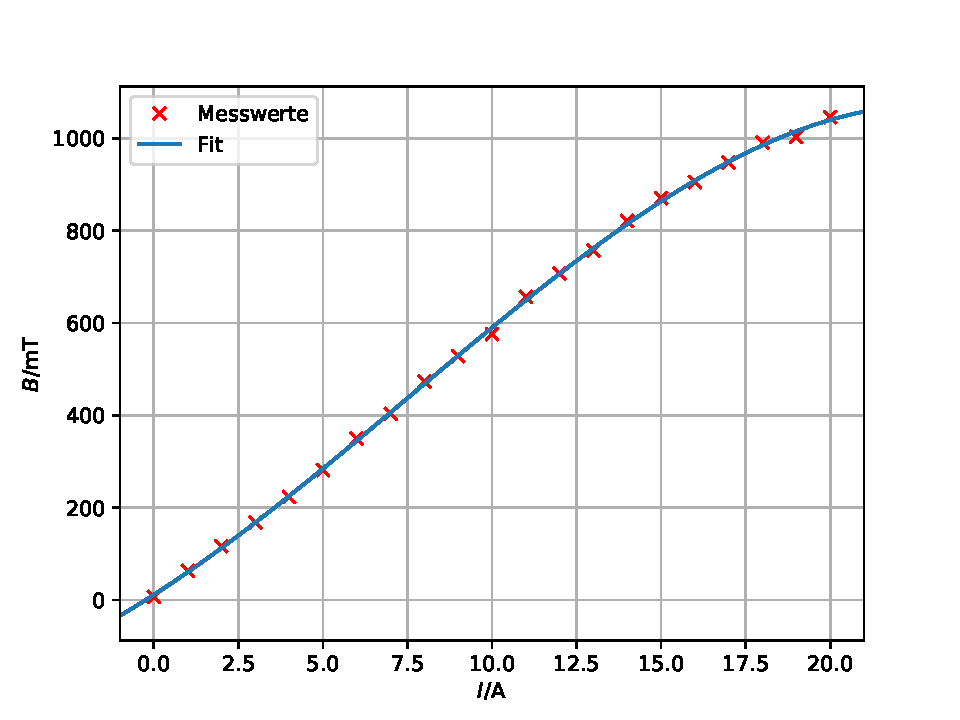
\includegraphics[width = \textwidth]{../Messdaten/plots/hysterese_absteigend.pdf}
  \caption{Absteigender Strom $I$.}
  \label{fig: hysterese_absteigend}
\end{subfigure}
\caption{Graphische Darstellung der Abhängigkeit $B(I)$ unter ab-/aufsteigendem Strom $I$ mit jeweiliger Regressionskurve.}
\label{fig: hysterese_fit}
\end{figure}
Im Folgenden wird Gleichung \eqref{eq: fitfuntion_hysterese} mit den Parametern \eqref{eq: params_up}
verwendet um den notwendigen Zusammenhang zwischen angelegtem Strom $I$ und magnetischer Flussdichte $B$ herzustellen. Der sehr geringe
$y$-Achsenabschnitt von $a_4 = \SI{3(6)}{\milli\tesla }$ wird vernachlässigt, sodass bei $I = \SI{0}{\ampere}$ von $B = \SI{0}{\tesla}$
ausgegangen werden kann.
